\documentclass[a4paper,12pt]{article}
\usepackage{styles}

\title{Analysis of FID shapes of Solids in glassy condition}
\author{Baranauskaite Valeriia, Mariia Ivanova, Leonid's Sister, Leonid Grunin}


\begin{document}


\section*{План статьи}
\subsection*{Введение}
\begin{enumerate}
  \item Какую информацию об образце мы можем получить, используя метод ЯМР в низких полях?
  \item О молекулярных движениях, как источнике информации, с точки зрения ЯМР-релаксометрии. О видах движения (работы Кая).
  \item О влиянии времени корреляции на T1, T2 твердых и жидких фаз образцов и форму спектральной линии.
  \item Корреляция структуры и свойств веществ с амплитудными и временными характеристиками спадов и параметров спектра.
  \item Микрообзор того, что кто смотрит по фиду.
  \item ГЭП – разброд и шатание в подходах к обработке фидов.
  \item Цель работы.
\end{enumerate}
\subsection*{Результаты и Дискуссия}
\begin{enumerate}
  \item Твердые тела. Подбор ЯМР-экспериментов с кратким описанием их особенностей.
  \item Обработка данных во временной области.
  \item Модели Абрагам, Гаусс, Вейбулл, Эксп. в зависимости от молекулярной динамики. Комбинации моделей в гетерофазных образцах. Модели не всегда идеально подходят – наши экспериментальные данные по разным видам твердых образцов.
  \item Обработка данных в частотной области.
  \item Формы спектральных линий. Второй момент. Взаимосвязь второго момента с временем поперечной релаксации.
  \item Новый метод: Second moment approximation.
  \item Идея.
  \item Примеры применения к спадам с осцилляцией и без.
  \item Сопоставление с результатами подходов Интегрирования и Усреднения.
  \item Возможные будущие задачи. Может, как-то корреляцию с DQ поизучать.
  \item Медленные движения молекул твердых тел эффективнее исследовать по спаду свободной индукции.
  \item Есть модификации как RK, Solid Echo (самые сильные дипольные взаимодействия), MSE (вроде, слабые).
  \item На каждом из упомянутых экспериментов по-разному отражается константа остаточных дипольных взаимодействий.
\end{enumerate}

\maketitle %to insert the title in the document
\section*{Abstract}

Why is it important\\
What has been done\\
What was found\\
What is the general result\\
How it can be used in the future\\

\newpage
\section{Introduction}\label{sec:Introduction}

The Time-Domain NMR (TD-NMR) signal of a sample provides quantitative information about its phase composition (rigid, soft, liquid), including the proportions and molecular mobility of these phases. 
FIDs can be processed using a range of well-developed approaches, including fitting, amplitude averaging, and transformation to the frequency domain, followed by subsequent calculations~\cite{Grunin2023}. 
\textcolor{red}{In many studies}, FIDs are analyzed by fitting predefined functions, typically based on NNLS algorithms. 
The choice of an appropriate model directly depends on the mobility regime of the molecules. 
Multiphase systems often produce multicomponent decays, which can be described by a sum of functions. 
These combinations are typically selected to minimize the number of variable parameters, which is necessary to improve the accuracy and repeatability of the approximation. 
\textcolor{red}{In most publications}, the signal parameters—such as amplitudes and NMR relaxation times—are related to the macroscopic properties of the samples. 
Moreover, probing these parameters can reveal the behavior of the system under controlled external effects and its evolution over time~\cite{vanRooyen2024}.

Several models are used to describe different mobility regimes: Abragamian, Pake, Gaussian, Weibullian, Exponential, and Stretched Exponential~\cite{Rntzsch2018}. 
The Abragamian function \((y(x) = A e^{-t^2/T_2^2} \cdot \frac{\sin(bx)}{bx})\) is frequently employed to represent the shape of transverse magnetization decays recorded in crystalline lattices, where a large number of interacting dipolar-coupled pairs are present \cite{Besghini2019}. 
Another model used to analyze contributions from molecules with highly restricted mobility is the Pake function, which, unlike the Abragamian model, incorporates the cosine function \((y(x) = A e^{-t^2/T_2^2} \cdot \cos \frac{bx}{2})\).
For certain types of samples, such as cellulose \cite{Grunin2017, Grunin2019}, the Pake model may yield better fitting results, as evidenced by a higher R². 
The Gaussian model \((y(x) = A e^{-t^2/T_2^2})\) is also suitable for describing signals from the solid phase, though it can be effective for soft-like systems as well. 
In general, the decays are modulated by the sample’s origin, particularly its structure.

A different set of equations defined as \((y(x) = A e^{-(t/T_2)^n})\) is characteristic of more isotropic dynamics []. 
The Weibullian function (or compressed exponential) \cite{Rntzsch2018} with \(1 < n < 2\) deconvolutes contributions primarily from soft- and liquid-like phases. The exponential model \((n = 1)\) is appropriate for molecules with high mobility and is especially effective when long components need to be subtracted. 
The stretched exponential model \((n < 1)\) indicates heterogeneous distributions of exponential decays, often due to inhomogeneities in the sample itself.

However, interpreting the data through fitting is not always reliable. 
In some specific cases, residual dipolar couplings in systems with anisotropic motions may lead to non-exponential decays []. 
Additionally, inaccuracies may arise from permanent magnet inhomogeneities. 
In polycrystalline samples, estimating interphase signals can be challenging because the signal may contribute to both rigid and soft phases \cite{Gorbunova2022}.

\newpage
\section{Experiment details}

\newpage
\section{Results and discussion}\label{sec:Results and discussion}
\subsection{FID processing in Time-Domain NMR}\label{sec:FID processing in Time-Domain NMR}

The recorded FID signal in NMR experiments typically consists of time, and real and imaginary components. 
Before analyzing the shape of FID, it undergoes preprocessing steps, including baseline subtraction, phase and frequency adjustments in the time domain.
The NMR signal for baseline is recorded in the empty ampule at exactly the same conditions as the sample. 
Phase adjustment addresses phase errors in the time domain data. 
These errors can arise from imperfections in the experimental setup or sample characteristics. 
The process involves finding the optimal phase angle that minimizes the difference between the real component of the FID signal and the overall amplitude of the signal within the initial part (typically before 30 microseconds). 
By adjusting the phase angle, we aim to align the real component of the signal with its amplitude, ensuring accurate representation of the signal's characteristics.

Frequency adjustment ensures that the frequency spectrum of the signal is correctly positioned and scaled.
This adjustment is crucial due to potential imperfections in the equipment or sample, which can cause the signal to deviate from its ideal state. 
The Fast Fourier Transform (FFT) procedure transforms the normalized time-domain signal into a frequency-domain in the form of a spectrum. 
The frequency axis is determined based on the time axis, following the Nyquist theorem. 
The spectrum is then shifted so that the maximum aligns with zero frequency, ensuring an even representation of positive and negative frequencies, i.e. symmetric spectrum. 
Finally, an inverse FFT (iFFT) is performed to obtain the FID signal with the corrected frequency.

\begin{figure}[H]
  \centering
  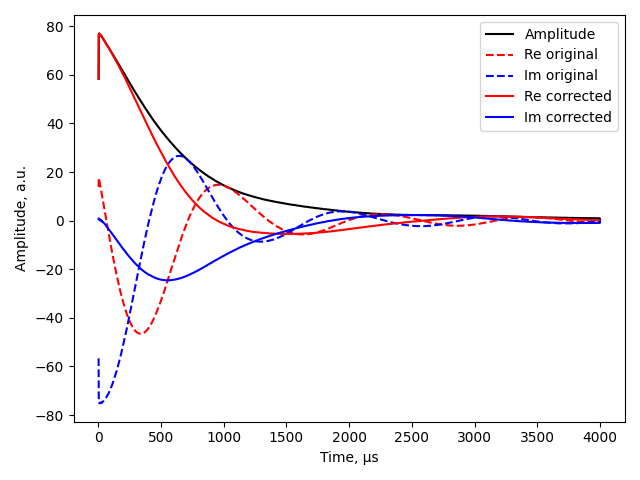
\includegraphics[width=10cm]{images/Original_Corrected_FID.png}
  \caption{The comparison between original (solid lines) and corrected (dashed lines) signals}
  \label{fig:Original_Corrected_FID}
\end{figure}

To mitigate the effects of magnet inhomogeneity at short time scales (before $30 \mu s$), where the fast relaxation occurs, it is recommended to subtract the long component. 
Glycerol, known for its long relaxation times, serves as a suitable reference. 
Alternatively, any substance with a transverse relaxation time exceeding 2 milliseconds can be used. 
The Glycerol's reference FID is normalized, adjusted for frequency and phase in the same manner as it was done with Sample. 
Subsequently, the real component of the Sample is divided by the amplitude of the Glycerol FID.

To eliminate the long component, an exponential fitting of the real part of the FID corresponding to the slow decay within the time range before $200 \mu s$ should be conducted and the fitted curve should be subtracted from the original data.

\begin{figure}[H]
  \centering
  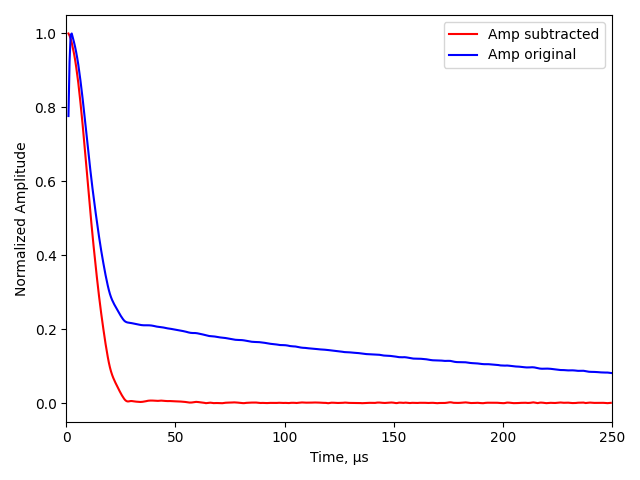
\includegraphics[width=10cm]{images/Subtracted_FID.png}
  \caption{The comparison of the original FID (red) and subtracted FID (blue)}
  \label{fig:Subtracted_FID}
\end{figure}

The concluding steps in the time-domain involve apodizing the real and imaginary components of the FID, followed by zero-filling to ensure that the final FID comprises a power of 2 number of data points ($2^n$). 
This step is crucial as FFT computation is more efficient with data containing this specific number of points. 
Subsequently, the FFT procedure is applied, yielding the resulting spectrum in the frequency-domain.

\begin{equation}
  \label{eq:apodization}
  f(apodization) = \exp\left(-\left[\frac{Time}{\sigma}\right]^4\right)
\end{equation}


\subsection{FID processing in Frequency-Domain NMR}\label{sec:FID processing in Frequency-Domain NMR}

The spectra derived from the FFT procedure can be manually phased using linear or polynomial functions.
Subsequently, the resulting real and imaginary components of the spectra can be recalculated accordingly. 

\begin{equation}
  \label{eq:amplitude calculation}
  \begin{split}
Re = Re \cdot \cos(\phi) - Im \cdot \sin(\phi)\\
Im = Re \cdot \sin(\phi) + Im \cdot \cos(\phi)\\
Amplitude = \sqrt{Re^2 + Im^2}
  \end{split}
\end{equation}

Additionally, apodization of the spectrum, akin to the time-domain signal, should be performed to ensure zero amplitude at high frequencies, utilizing similar equations as in \cref{eq:apodization}. 
Once apodized, the acquired spectrum is prepared for further analysis, such as the calculation of the second moment.

\section{SE and FID}\label{sec:SE and FID}

In the analysis of Solid Echo (SE) and Free Induction Decay (FID) signals, several steps are undertaken to ensure precise data acquisition, correction, and interpretation as is described in \cref{sec:FID processing in Time-Domain NMR,sec:FID processing in Frequency-Domain NMR}.
The SE signals and FID are shown in \cref{fig:FID_SE} a).
The maxima of the SE signals are then plotted versus corresponding echo times as shown in \cref{fig:FID_SE} b).
To interpret the data, a Gaussian function is employed for fitting. 

\begin{equation}
  \label{eq:gaussian}
  G(x) = A \cdot \exp\left(-\frac{x^2}{2\sigma^2}\right)
\end{equation}

The Gaussian function is of the standard form, where the key parameter $A$ represents the amplitude. 
This value is directly derived from the SE signals and offers an essential reference for later stages of the analysis.

\begin{figure}[H]
  \centering
  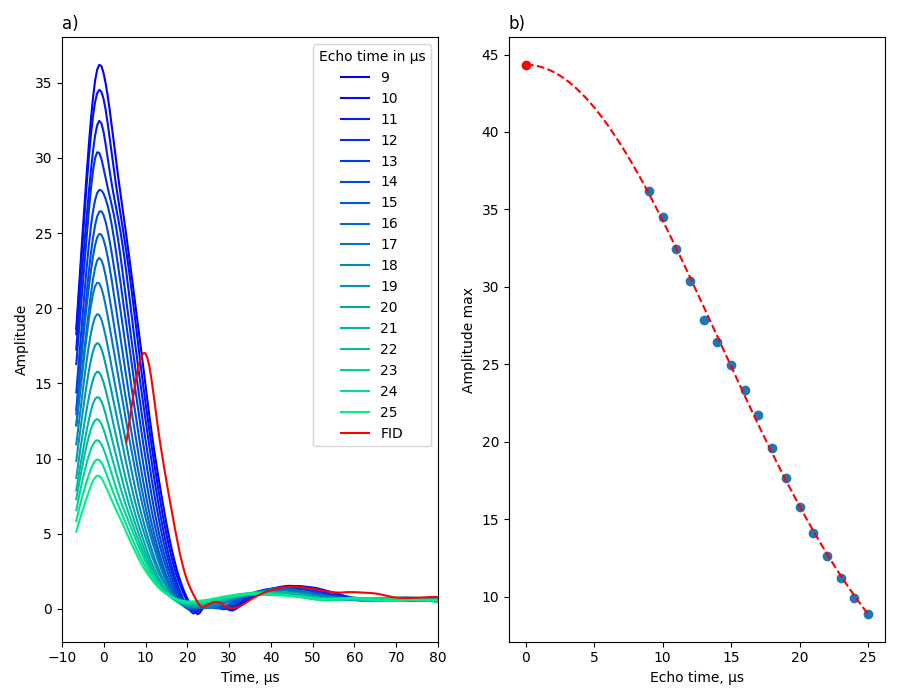
\includegraphics[width=10cm]{images/FID_SE.png}
  \caption{a: The overall representation of SE signals and FID (red); b: The SE maxima versus the corresponding echo times}
  \label{fig:FID_SE}
\end{figure}

Next, the initial portion of the FID signal, particularly the segment between 10 and 20 microseconds is fitted using the same Gaussian model employed earlier for the SE \cref{eq:gaussian}. 
It is crucial to ensure that the amplitude of the Gaussian fit matches the maximum amplitude observed at time $t = 0$, as derived from the SE signal maxima.
After fitting the FID signal, intersection points between the fitted Gaussian curve and the original FID signal are determined. 
These intersection points highlight critical aspects of the experimental data and assist in reconstructing the hidden portions of the FID using the fitted Gaussian model \cref{fig:Rebuild_FID}.

\begin{figure}[H]
  \centering
  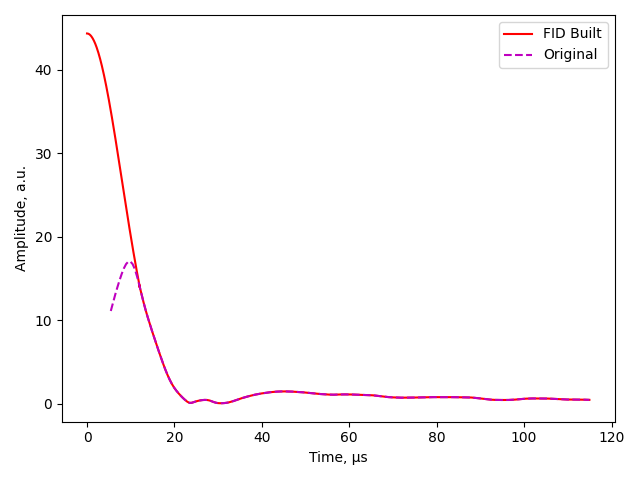
\includegraphics[width=10cm]{images/Rebuild_FID.png}
  \caption{The rebuild FID and the original FID}
  \label{fig:Rebuild_FID}
\end{figure}

The final step involves validating the amplitude of the FID, which is rebuilt from the SE maxima. To ensure the accuracy of this reconstruction, the FID of a water sample with a known mass is recorded under identical experimental conditions. The maximum amplitudes of the FIDs for both the water and the cellulose samples are then compared, as these amplitudes correspond directly to the number of protons in each sample. The proton density, calculated using the formula:

\begin{equation}
  \label{eq:proton_density}
  \text{Proton density} = \frac{\text{max(Amplitude)}}{ \left(\frac{\text{mass}}{M}\right) \cdot N_A \cdot \text{(number of protons per molecule)} }
\end{equation}

This formula provides a reference value for the proton density. 
By multiplying the proton density obtained from the water sample by the number of protons in the cellulose sample, a reference value of 42 is obtained. 
This reference is then compared to the maximum amplitude of 44 from the rebuilt FID. 
The close agreement between these values, within the margin of error, confirms the reliability of the proposed method for reconstructing the FID from SE signals.

\begin{figure}[H]
  \centering
  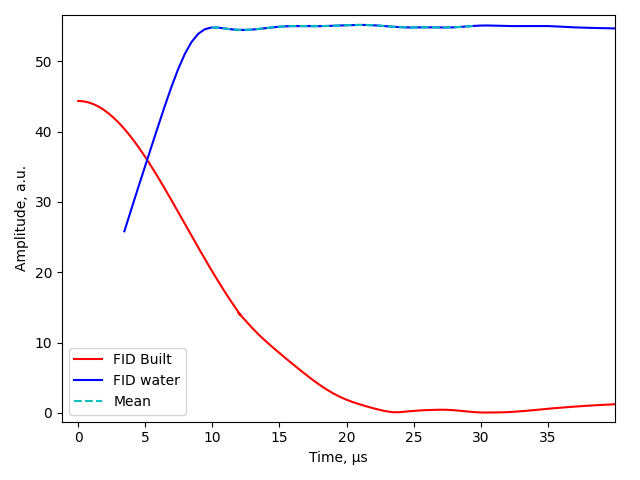
\includegraphics[width=10cm]{images/Water_Cell_FID.png}
  \caption{The recorded FID of water and cellulose sample}
  \label{fig:Water_Cell_FID}
\end{figure}

\begin{table}[h]
  \centering
  \begin{tabular}{|l|c|c|c|c|}
  \hline
  \textbf{Compound} & \textbf{Mass (g)} & \textbf{Molar Mass (g/mol)} & \textbf{Proton Density (e-21)} & \textbf{FID Max Amplitude} \\ \hline
  \textbf{Water}    & 0.0963            & 18.01528                    & 8.522                         & 55                         \\ \hline
  \textbf{Cellulose} & 0.1334           & 162.1406                    & 8.949                         & 44                         \\ \hline
  \end{tabular}
  \caption{Physical properties and FID amplitudes of Water and Cellulose samples}
  \label{tab:fid_data}
  \end{table}
  

\newpage
\section{Conclusions}

\newpage
\printbibliography

\end{document}
